\documentclass{ExcelAtFIT}
\usepackage[T1]{fontenc}
%\documentclass[czech]{ExcelAtFIT} % when writing in CZECH
%\documentclass[slovak]{ExcelAtFIT} % when writing in SLOVAK


%--------------------------------------------------------
%--------------------------------------------------------
%	REVIEW vs. FINAL VERSION
%--------------------------------------------------------

%   LEAVE this line commented out for the REVIEW VERSIONS
%   UNCOMMENT this line to get the FINAL VERSION
%\ExcelFinalCopy


%--------------------------------------------------------
%--------------------------------------------------------
%	PDF CUSTOMIZATION
%--------------------------------------------------------

\hypersetup{
	pdftitle={Paper Title},
	pdfauthor={Jakub Fajkus},
	pdfkeywords={Keyword1, Keyword2, Keyword3}
}

%--------------------------------------------------------
%--------------------------------------------------------
%	ARTICLE INFORMATION
%--------------------------------------------------------

\ExcelYear{2018}

\PaperTitle{How to Write an Excellent Excel@FIT Paper}

\Authors{Adam Herout*}
\affiliation{*%
  \href{mailto:herout@fit.vutbr.cz}{herout@fit.vutbr.cz},
  \textit{Faculty of Information Technology, Brno University of Technology}}

\Keywords{Evolutionary computation --- Neural Networks --- Linear Genetic Programming --- Robotics}

\Supplementary{\href{http://youtu.be/S3msCdn3fNM}{Demonstration Video} --- \href{http://excel.fit.vutbr.cz/}{Downloadable Code}}


%--------------------------------------------------------
%--------------------------------------------------------
%	ABSTRACT and TEASER
%--------------------------------------------------------

\Abstract{
Tato prace se zabyva navrhem a pouzitim frameworku vyuzivajici Evolucni Algoritmy, ktery bude pouzit pro hledani zpusobu rizeni pocitacoveho
modelu jednoducheho autonomniho robota. Tento model bude v pocitacove simulaci vykonavat netrivialni pohyb.
Pro řízení modelu robota jsou použity dva rozdílné přístupy.
První přístup je založen na instrukcích, odpovidajici Linearnimu Genetickemu Programovani.
Druhý přístup využívá feedforward neuronové sítě.
Oba pristupy jsou podrobeny nekolika experimentum, ktere overuji jejich vhodnost pro dany typ problemu.
Pro dany problem je provedeno experimentalni srovani ruznych instanci EA.
Nasledne jsou pristupy vyhodnoceny a diskutovany vysledky s durazem na porovnani obou pristupu.
Vysledky prace potrvzuji, ze komplexnejsi chovani vyzaduje jistou miru samoadaptace(environment awarness) a ze je toto
mozne dosahnout obema zvolenymi pristupy.
}

\Teaser{
	\TeaserImage{placeholder.pdf}
	\TeaserImage{placeholder.pdf}
	\TeaserImage{placeholder.pdf}
}



%--------------------------------------------------------
%--------------------------------------------------------
%--------------------------------------------------------
%--------------------------------------------------------
\begin{document}

\startdocument


%--------------------------------------------------------
%--------------------------------------------------------
%	ARTICLE CONTENTS
%--------------------------------------------------------

%--------------------------------------------------------
%--------------------------------------------------------
%--------------------------------------------------------
%--------------------------------------------------------
\section{Introduction}

\todo{asi bych prevzal uvod do nejake robotiky}
V oblasti robotiky je velmi dulezita schopnost rychle a levne prototypovat mozna reseni.
K tomuto ucelu je velmi vhodne pouziti pocitacove modelovani a simulace.
V situaci, kdy mame navrzenou fyzickou stranku robota, nastava otazka, jak rychle prototypovat jeho rizeni.
Existuje mnoho moznosti realizace rizeni robota, lisici se v zavislosti na pozadavcich a povaze cinosti robota.
Rizeni robota muze byt zalozeno na instrukcich nejakeho imperativniho jazyka nebo na neuronovych sitich.
Dalsi z moznosti jsou ruzne planovaci algoritmy a systemy. \todo{citace, zdroje, terminologie}
Pro prototypovani je vyhodne mit nastroj, ktery je schopny hledat vyhodne zpusoby rizeni robota.
Evolutionary algorithms are good for this purpose, because they are applicable for a wide range of problems.

Hledame reseni pro problem, ktery je definovan takto.
Mame model jednoducheho robota, ktery je castecne inspirovany prirodou(mravenec). \todo{viz obr.}
Cilem je nalezt program(posloupnost instrukci) nebo konfiguraci neuronove site tak, aby model robota vykonaval dany netrivialni pohyb(po primce a spirale).
Hledame tedy jiste reseni.
Hledani reseni probiha automatizovane s vyuzitim evolucnich algoritmu.
Algoritmy pomoci evoluce vyvijeji program, nebo neuronovou sit tak, aby se robot pohyboval po pozadovane trajektorii.
K vyhodnoceni uspesnosti reseni je pouzit fyzikalni simulator specializovany na simulaci robotu Mujoco\cite{Todorov2012}.

There is many works focused on evolutionary robotics.
The ones that were focusing robot control were using many techniques, including finite state machines\cite{Hodgins1996}, classical control theory\cite{Mita1984} and neural networks \cite{Reil2002}\cite{Lewis1996}.
There is also a number of works using Evolutionary Algorithms to evolve controllers, particularly neural networks\cite{Randall1992}\cite{Farooq2013}.
There are also works that are using Genetic Programming\cite{Macedo2017}. The most similar work to ours is the work of Wollf and Mattias\cite{Wolff2007}. They are using Linear Genetic Programming to evolve a bipedal motion of a humanoid model.

Our work, as well as work of Wollf and Mattias, is using LGP, with similar interpret structure, but with different approach to program structure.
Our approach splits the program into smaller subprograms, as opposed to one program.
Our instruction set is also reduced and the arithmetic of the interpret are different.
Both the works use some sort of a environmental awareness.
Our work implements that by introducing an event subprogram, which is executed when an event occurs in the environment(coming closer to a reference point).
No sensory information is used.
Wollf and Mattias used a set of sensors, that are measuring current joint angles of the model.

This work offers an approach using the subprograms and reduced instruction set.
This approach is simple both to implement and evolve.
Cost for that is a reduced environment awareness, as the program does not have a knowledge about its environment but it is rather controlled from the outside.
This could be used with a combination of some kind of "brain" having a better environment awareness.
The "brain" would decide, which program will be run.


%--------------------------------------------------------
%--------------------------------------------------------
%--------------------------------------------------------
%--------------------------------------------------------
\section{Teoreticky uvod}
\label{sec:theory}
\todo{Zde bude kratky teoreticky uvod k EA a LGP}

%--------------------------------------------------------
%--------------------------------------------------------
%--------------------------------------------------------
%--------------------------------------------------------

\section{Framework architecture and implementation}
\label{sec:ArchitectureAndImplementation}
{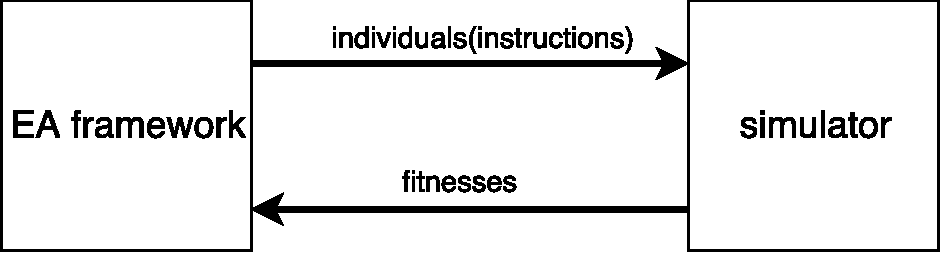
\includegraphics[height=5.8em]{top_level_architecture.pdf}
\todo{misto fitness psat o objective function?}
System je rozdelen na dve aplikace.
Hlavni aplikaci je EA framework, ktery zajistuje vsechnu praci s evoluci.
Druhou casti systemu je simulator Mujoco, ktery je doplnen vlastnim kodem, ktery zajistuje prevod instrukci na vstupy simulatoru a pocita objective function.
Propojeni techto dvou aplikaci je realizovano pres systemova volani pro spousteni procesu pres shell.

V simulatoru je pripravena scena, ve ktere je umisten model robota a mnozina referencnich bodu, ktere jsou umisteny na spirale.
Robot ma za ukol se pohybovat ve scene tak, ze se ke vsem referencnim bodum priblizi co nejvice.
Timto robot vykonava pohyb po dane trajektorii.

\subsection{Realizace rizeni robota}
Rizeni robota je realizovano pomoci jednoduchych instrukci.
V simulatoru je zabudovat interpret, ktery je schopny tyto instrukce prevadet na signaly, ktere zpracovava simulator.
Tyto signaly rikaji, jaka sila se bude aplikovat v jednotlivych kloubech modelu robota.
Interpret pracuje pouze s celymi cisly, a to od -5 do 5 vcetne.

Interpret obsahuje predem dany pocet vnitrnich pametovych mist(vnitrni registry), ktere je mozne modifikovat za pouziti instrukci.
Interpret take obsahuje vystupni pametova mista(vystupni registry).
Kazdy vystupni registr je prirazen k jednomu kloubu robota.
Hodnoty v techto registrech jsou prevadeny na intenzitu sily, ktera bude v techto kloubech pusobit.

Program se sklada z instrukci, ktere meni stav vnitrnich registru a stav vnejsich registru.
Tyto instrukce jsou vypsany v Table~\ref{tab:Instructions}.

Program je rozdelen do tri podprogramu - init, event a main.
Init program je proveden v nulovem case a to pouze po spusteni simulace.
Slouzi k nastaveni pocatecniho stavu vnitrnich registru. Jsou zde povoleny jen instrukce SRE a SOV\@.

Dalsim podprogramem je event.
Ten je spousten pokazde, kdyz se model robota dostatecne priblizi k nekteremu z referencnich bodu(pro kazdy bod ale pouze jednou).
Vsechny instrukce jsou provedeny v nulovem case, stejne jako v init podprogramu.
Tento podprogram slouzi ke zmene vnitrich registru.
Jsou zde povoleny instrukce SRE, SOV, INC, DEC

Hlavnim podprogramem je main.
Tento podprogram je provaden v nekonecne smycce.
Zde probiha kopirovani hodnot z vnitrnich registru do vystupnich registru.
Instrukce zde nejsou provadeny v nulovem case, ale casovy rozestup mezi nimi je 0.5 sekundy.
Jsou zde povoleny instrukce SOU, SOV.


\begin{table}[h]
	\caption{Instructions of the interpret}
	\vspace{1em}
\caption*{
INC increments an internal register by a given constant.
DEC decrements an internal register by a given constant.
SOU copies an internal register value to a output register.
SOV copies a constant value to a output register.
SRE copies a constant to an internal register.
}
	\begin{tabular}{l|{c}|r}
		\textbf{Instruction}    & \textbf{Parameter 1} & \textbf{Parameter 2}    \\
		\hline
		INC                     & Internal register    & Constant        \\
		DEC                     & Internal register    & Constant        \\
		SOU                     & Internal register    & Output register \\
		SOV                     & Constant             & Output register \\
		SRE                     & Internal register    & Constant        \\
	\end{tabular}
	\label{tab:Instructions}
\end{table}


%--------------------------------------------------------
%--------------------------------------------------------
%--------------------------------------------------------
%--------------------------------------------------------
\section{Experiements}
\label{sec:Experiments}
Zde popiseme jednitlive experimenty a nastaveni EA, ktere bylo pouzito.

\subsection{Experiment overview}
\todo{Zde bude popis experimentu - mravenec na primce? a na spirale}
\todo{Vsechny informace k experiemntu: tj. konfigurace GA, delka programu, rozdeleni na podprogramy(kolik kam), delka simulace}

\subsection{Results}
\todo{Zde budou prehledne vysledky experimentu - grafy, cisla, tabulky, obrazky, vsechno}
%--------------------------------------------------------
%--------------------------------------------------------
%--------------------------------------------------------
%--------------------------------------------------------

\section{Conclusions}
\label{sec:Conclusions}

\textbf{[Paper Summary]} What was the paper about, then? What the reader needs to remember about it?
Tato prace ukazala pouziti evolucnich algoritmu pro hledani programu pro rizeni robota. \todo{neco dalsiho}

\textbf{[Highlights of Results]} Exact numbers. Remind the reader that the paper matters.
\phony{Lorem ipsum dolor sit amet, consectetur adipiscing elit. Sed tempus fermentum ipsum at venenatis. Curabitur ultricies, mauris eu ullamcorper mattis, ligula purus dapibus mi, vel dapibus odio nulla et ex. Sed viverra cursus mattis. Suspendisse ornare semper condimentum. Interdum et malesuada fames ac ante ipsum.}

\textbf{[Paper Contributions]} What is the original contribution of this work? Two or three thoughts that one should definitely take home.
\phony{Lorem ipsum dolor sit amet, consectetur adipiscing elit. Praesent posuere mattis ante at imperdiet. Cras id tincidunt purus. Aliquam erat volutpat. Morbi non gravida nisi, non iaculis tortor. Quisque at fringilla neque.}

\textbf{[Future Work]} How can other researchers / developers make use of the results of this work?  Do you have further plans with this work? Or anybody else?
\phony{Lorem ipsum dolor sit amet, consectetur adipiscing elit. Suspendisse sollicitudin posuere massa, non convallis purus ultricies sit amet. Duis at nisl tincidunt, maximus risus a, aliquet massa. Vestibulum libero odio, condimentum ut ex non, eleifend.}

\section*{Acknowledgements}
I would like to thank my supervisor X. Y. for his help.

%--------------------------------------------------------
%--------------------------------------------------------
%--------------------------------------------------------
%	REFERENCE LIST
%--------------------------------------------------------
%--------------------------------------------------------
\phantomsection
\bibliographystyle{unsrt}
\bibliography{2018-ExcelFIT-ShortName-bib}

%--------------------------------------------------------
%--------------------------------------------------------
%--------------------------------------------------------
\end{document}
